% In this section you should present the results and main findings from your project.
\chapter{Results}

This chapter presents the final results from the supervised and unsupervised model methods applied in the project. Detailed results, including visualizations and tables, are provided for clarity.

\section{Unsupervised models}

\subsection{Scalable clustering models}
\subsubsection{a. LDA with Term-Frequency (TF)}
\subsubsection{b. K-Means with ClinicalBERT embeddings}
Topic modeling using LDA was used for sentence embeddings to discover latent patterns in the data. Additionally, semantic clusters were made with K-Means clustering on ClinicalBERT embeddings of the data. Both these algorithms enable evaluation of the model for large amounts of the dataset. Performance was evaluated using perplexity and silhouette scores with varying different number of topic clusters (k) to circumvent the unreliability in the manually annotated dataset.

Table \ref{tab:lda-kmeans-results} showcases the performance of both these algorithms.
\begin{table}[H]
\centering
\caption{LDA and K-Means: Perplexity and Silhouette Scores}
\label{tab:lda-kmeans-results}
\begin{tabular}{lccc}
\toprule
\textbf{Algorithm} & \textbf{Number of Clusters (k)} & \textbf{Perplexity} & \textbf{Silhouette Score} \\
\midrule
LDA & 4 & 7.1100 & 0.7198 \\[0.5ex]
LDA & 5 & 7.3004 & 0.7200 \\[0.5ex]
LDA & 6 & 7.5069 & 0.7115 \\[0.5ex]
KMeans & 3 & -- & 0.0555 \\[0.5ex]
KMeans & 4 & -- & 0.0494 \\[0.5ex]
KMeans & 5 & -- & 0.0549 \\
\bottomrule
\end{tabular}
\end{table}

Two word clouds for the semantic clustering with K-Means is shown in \ref{fig:lda-kmeans-wordclouds-1-3} illustrate clear differences in the coherence and thematic focus of clustered sentence groups. The first word cloud (Topic 2) demonstrates strong semantic cohesion around the Communication and Cognition domain. Terms such as level, mental, alert, interactive, consciousness, and coherent are indicative of clinical descriptions related to cognitive and communicative status. This suggests that the clustering algorithm effectively isolated a group of sentences that share consistent linguistic patterns and are likely associated with the ICF Communication/Cognition category.

In contrast, the second word cloud lacks a similarly coherent thematic focus. While it contains terms such as Admission, Medication, and Discharge, there is no apparent dominant lexical pattern corresponding to a single functional status category. This may reflect either limitations in the clustering and embedding technique or overlapping semantic content across multiple clinical categories, which challenges the effectiveness of unsupervised clustering for such cases.

\begin{figure}[H]
\centering
\begin{subfigure}{0.45\textwidth}
  \centering
  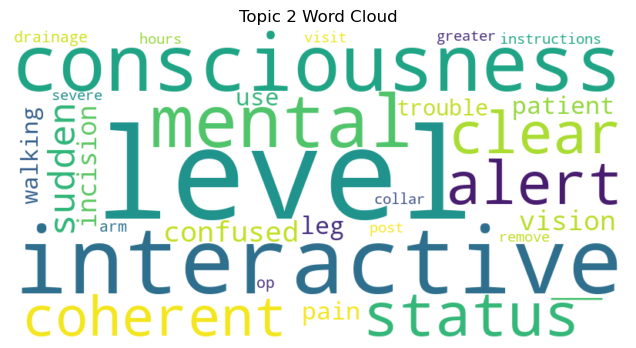
\includegraphics[width=\linewidth]{images/Unsupervised_Results/wordcloud_cluster_1.png}
  \subcaption{This topic cluster consists largely of documents pertaining to the ICF category COM/COG.}
\end{subfigure}
\hfill
\begin{subfigure}{0.45\textwidth}
  \centering
  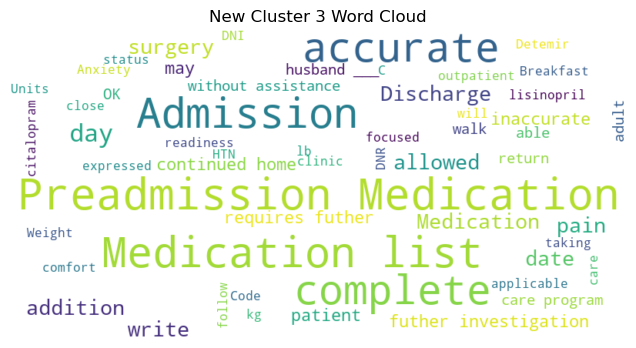
\includegraphics[width=\linewidth]{images/Unsupervised_Results/wordcloud_cluster_3.png}
  \subcaption{This cluster does not appear to contain a dominant semantic theme.}
\end{subfigure}
\caption{Word Clouds for select clusters from K-Means with ClinicalBERT embeddings.}
\label{fig:lda-kmeans-wordclouds-1-3}
\end{figure}

\subsection{Rule-Based with K-Means}

In this approach, a hybrid rule-based system combined with KMeans-based auto-labelling was employed to extract sentences potentially containing functional status information (FSI). The results presented below reflect outcomes from manual inspection and contextual analysis of the labelled outputs.

\begin{table}[H]
\centering
\caption{Manual Inspection of Cluster Labels by ICF Category}
\label{tab:manual-inspection}
\resizebox{\textwidth}{!}{%
\begin{tabular}{lcccc}
\toprule
\textbf{ICF Category} & \textbf{Correct Label (\%)} & \textbf{Contextually Misleading (\%)} & \textbf{Incorrect (\%)} & \textbf{Total Sentences} \\
\midrule
Mobility & 70 & 20 & 10 & 1430 \\[0.5ex]
SCDL & 60 & 30 & 10 & 1149 \\[0.5ex]
IPIR & 30 & 60 & 10 & 870 \\[0.5ex]
COM/COG & 80 & 10 & 10 & 346 \\ 
\bottomrule
\end{tabular}%
}
\end{table}

\begin{figure}[H]
\centering
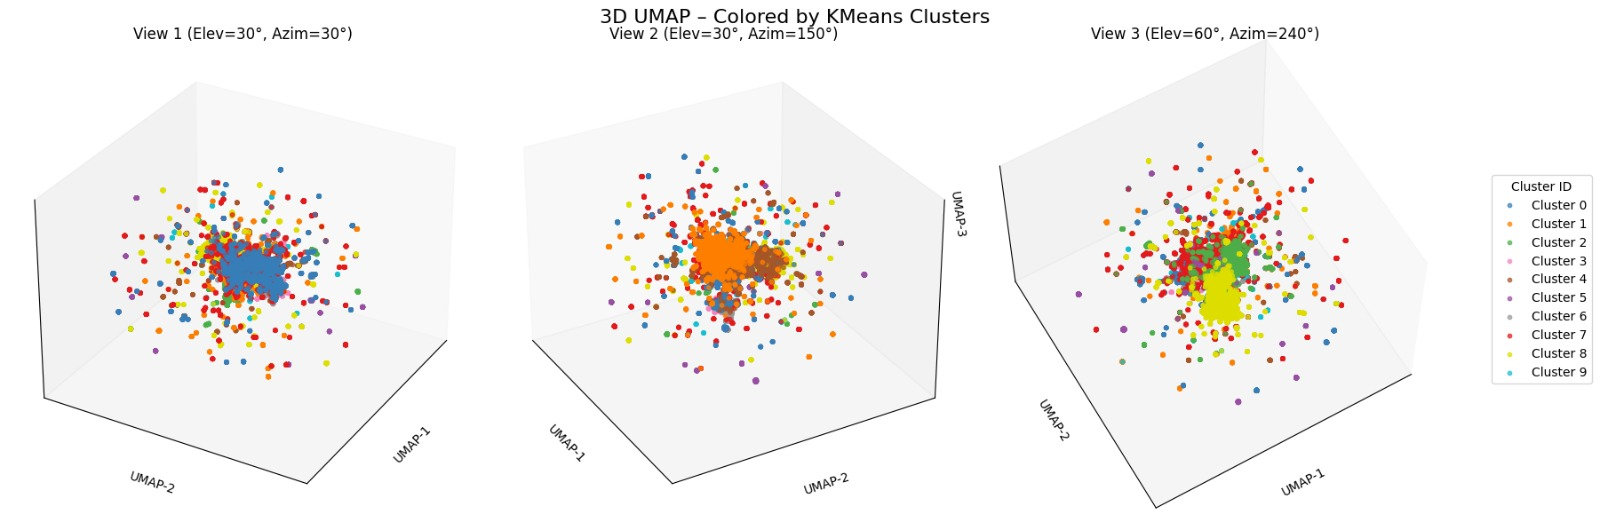
\includegraphics[width=\textwidth]{images/Unsupervised_Results/rulebased_umap_clusters.jpg}
\caption{3D UMAP Visualization of Rule-Based Sentences Colored by K-Means Clusters}
\label{fig:rulebased-kmeans-umap}
\end{figure}

\begin{figure}[H]
\centering
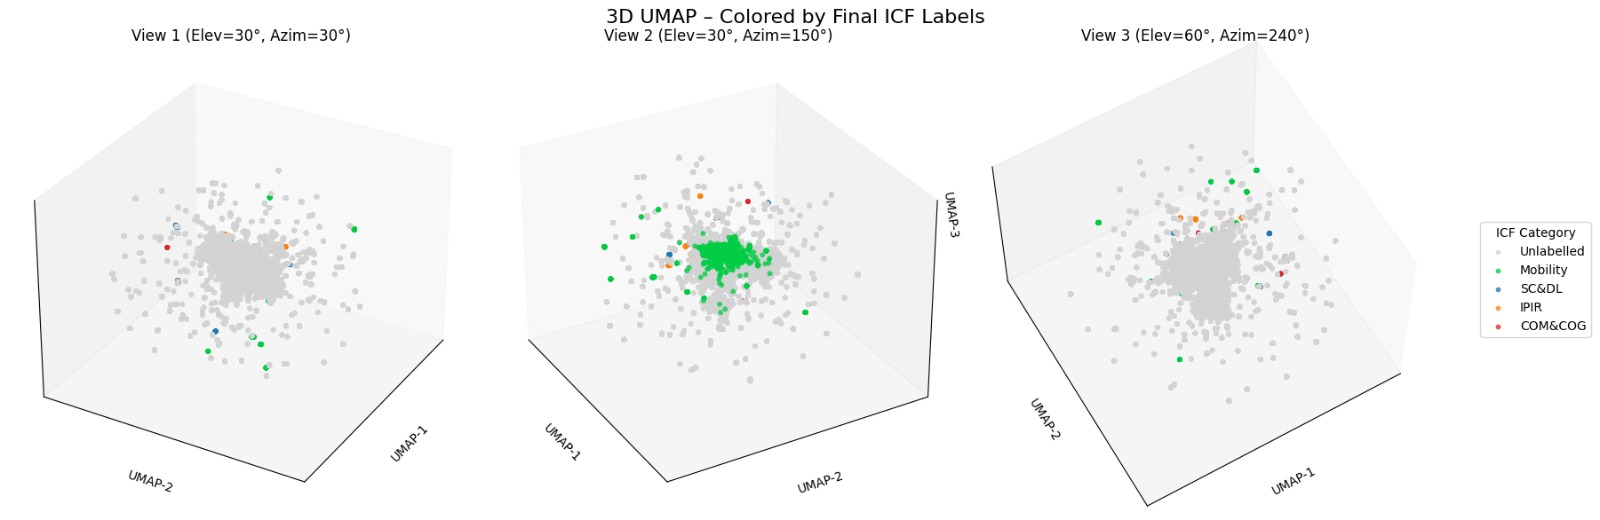
\includegraphics[width=\textwidth]{images/Unsupervised_Results/rulebased_umap_icf_labels.jpg}
\caption{3D UMAP Visualization of Final ICF Domain Labels Assigned to Clusters}
\label{fig:rulebased-umap-icf}
\end{figure}

\begin{figure}[H]
\centering
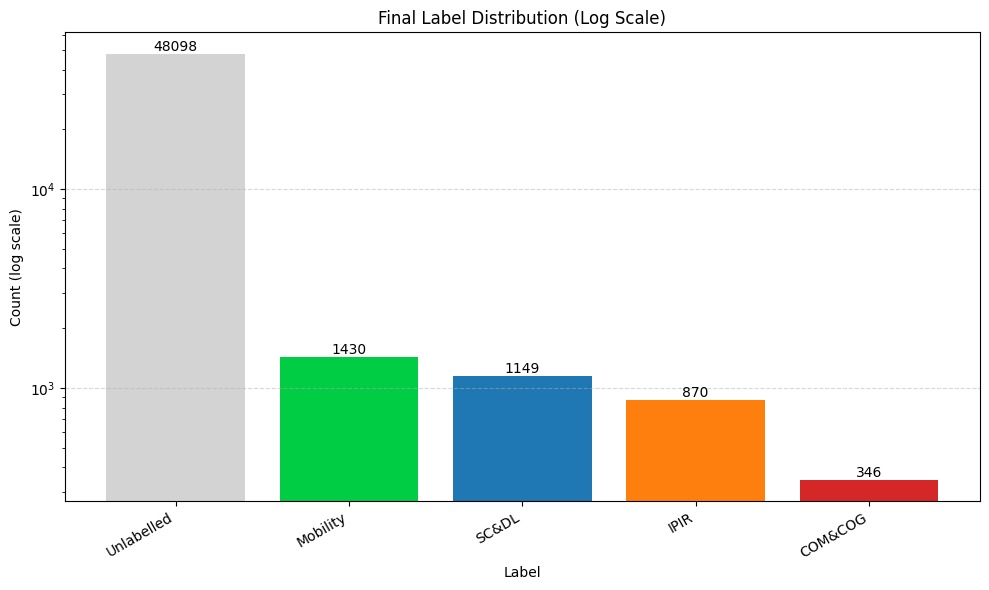
\includegraphics[width=0.65\textwidth]{images/Unsupervised_Results/rulebased_icf_distribution.jpg}
\caption{Final Label Distribution Across ICF Categories (Log Scale)}
\label{fig:rulebased-icf-distribution}
\end{figure}

\vspace{0.5cm}

\begin{table}[H]
\centering
\caption{Precision and Error Summary for Rule-Based with K-Means}
\label{tab:precision-summary}
\begin{tabular}{l c p{8cm}}  % Adjust the width of the last column as needed
\toprule
\textbf{ICF Category} & \textbf{Precision Strength} & \textbf{Main Error Source} \\
\midrule
Mobility & High & Overfitting to generic words like ``run'', ``walk'' \\
SCDL & Moderate & Vague phrases without clear context \\
IPIR & Low & Misclassification on words such as ``family'', ``spouse'' with no interactive context \\
COM/COG & High & Minimal ambiguity \\
\bottomrule
\end{tabular}
\end{table}

\paragraph{Mobility:} Mobility had the highest visibility when it comes to lexical patterns, which explains strong performance. However, overreliance on keywords and phrases, and other surface terms caused conceptual mismatches.

\paragraph{SCDL:} The SCDL dictionary consisted of broad terms which matched some irrelevant medical or procedural language. Semantic embeddings helped slightly, but higher ambiguity remains without sentence-level embeddings.

\paragraph{IPIR:} IPIR suffered heavily due to semantic drift. The term-based approach triggered on certain keywords without ensuring interactional context, which is necessary for a sentence to be classified as IPIR. Hence, clustering amplified this by grouping such mentions and many sentences were wrongly labelled.

\paragraph{Communication and Cognition:} Despite being the category with the lowest number of sentences labelled, COM/COG showed high precision. This is likely due to the well-defined keywords list, which includes words such as \textit{speaking, reading, thinking, etc.}, which co-occur with clinically meaningful context and are picked up well by the model.

\section{Supervised}

\subsection{CNN-RNN}

The CNN-RNN model achieved a micro-F1 score of \textbf{0.7403} and a macro-F1 score of \textbf{0.7294}. Per-class metrics are reported in Table~\ref{tab:supervised-results}.

\begin{table}[H]
\centering
\caption{Detailed Classification Results for CNN-RNN Model}
\label{tab:supervised-results}
\begin{tabular}{lccccccc}
\toprule
\textbf{ICF Domain} & \textbf{TN} & \textbf{FP} & \textbf{FN} & \textbf{TP} & \textbf{Precision} & \textbf{Recall} \\ 
\midrule
Mobility & 870 & 45 & 49 & 207 & 0.8214 & 0.8086\\[0.5ex]
Self-care/Domestic life & 903 & 36 & 74 & 158 & 0.8144 & 0.6810\\[0.5ex]
Interpersonal interactions & 954 & 49 & 61 & 107 & 0.6859 & 0.6369\\[0.5ex]
Communication/Cognition & 965 & 34 & 61 & 111 & 0.7655 & 0.6453\\ 
\bottomrule
\end{tabular}
\end{table}

\begin{figure}[H]
\centering
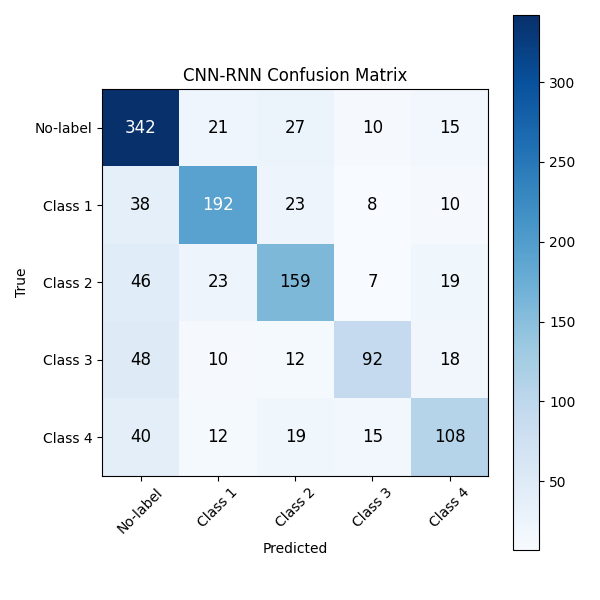
\includegraphics[width=0.6\textwidth]{images/Supervised_Results/cnn-rnn_confusion_matrix.png}
\caption{Confusion Matrix for the CNN-RNN Model}
\label{fig:cnn-rnn-confusion-matrix}
\end{figure}

\begin{figure}[H]
\centering
\begin{minipage}[b]{0.48\textwidth}
    \centering
    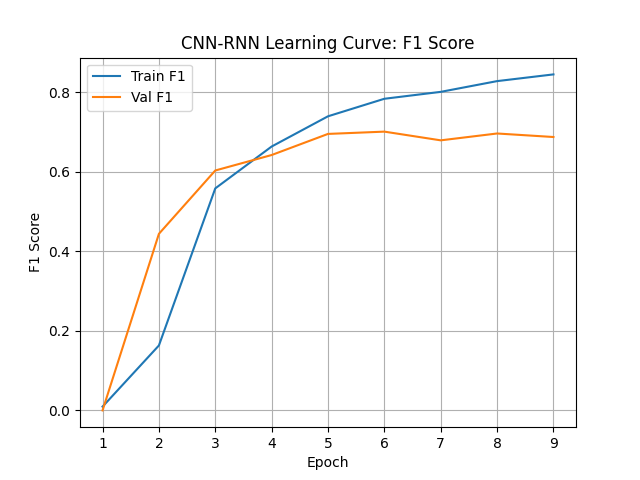
\includegraphics[width=\textwidth]{images/Supervised_Results/cnn-rnn_learning_curve_f1.png}
    \caption{Learning Curve (F1-Score) for the CNN-RNN Model}
    \label{fig:cnn-rnn-learning-curve-f1}
\end{minipage}
\hfill
\begin{minipage}[b]{0.48\textwidth}
    \centering
    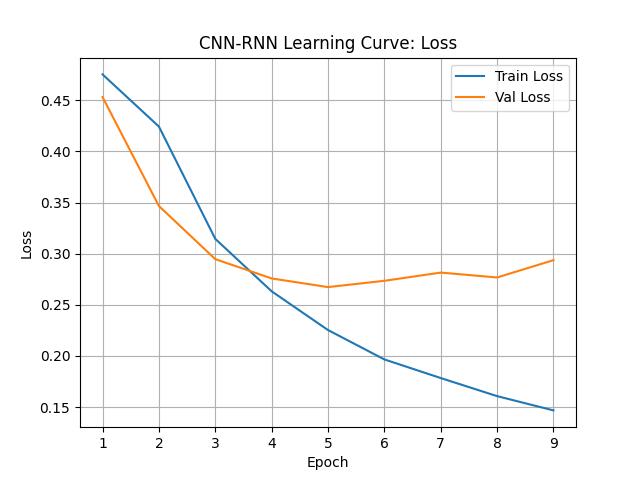
\includegraphics[width=\textwidth]{images/Supervised_Results/cnn-rnn_learning_curve_loss.png}
    \caption{Learning Curve (Loss) for the CNN-RNN Model}
    \label{fig:cnn-rnn-learning-curve-loss}
\end{minipage}
\end{figure}

\vspace{1em} 
\subsection{FNN}

The FNN model reached a micro-F1 score of \textbf{0.6713} and macro-F1 score of \textbf{0.6611}. Detailed results for each class are presented in Table~\ref{tab:fnn-results}.

\begin{table}[H]
\centering
\caption{Detailed Classification Results for FNN Model}
\label{tab:fnn-results}
\begin{tabular}{lccccccc}
\toprule
\textbf{ICF Domain} & \textbf{TN} & \textbf{FP} & \textbf{FN} & \textbf{TP} & \textbf{Precision} & \textbf{Recall} \\ 
\midrule
Mobility & 854 & 61 & 75 & 181 & 0.7479 & 0.7070 \\
Self-care/Domestic life & 872 & 67 & 76 & 156 & 0.6996 & 0.6724 \\
Interpersonal interactions & 952 & 51 & 71 & 97 & 0.6554 & 0.5774 \\
Communication/Cognition & 963 & 36 & 79 & 93 & 0.7209 & 0.5407 \\
\bottomrule
\end{tabular}
\end{table}

\begin{figure}[H]
\centering
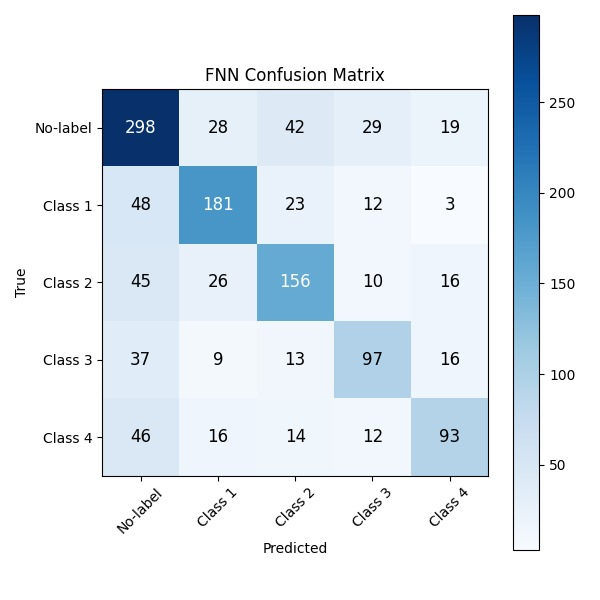
\includegraphics[width=0.6\textwidth]{images/Supervised_Results/FNN_confusion_matrix.jpg}
\caption{Confusion Matrix for the FNN Model}
\label{fig:fnn-confusion}
\end{figure}

\begin{figure}[H]
\centering
\begin{minipage}[b]{0.48\textwidth}
    \centering
    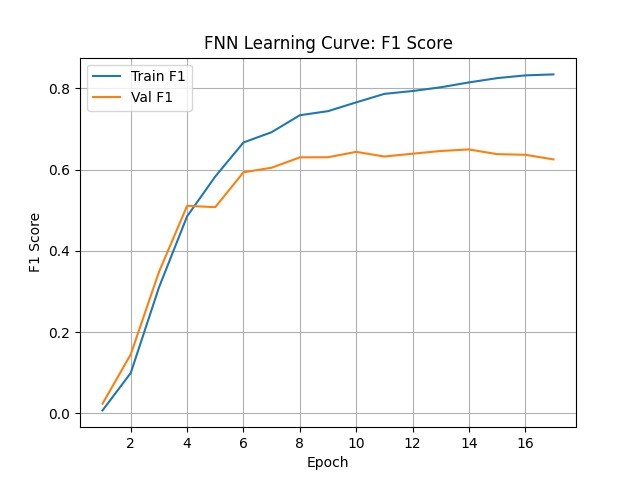
\includegraphics[width=\textwidth]{images/Supervised_Results/FNN_learningcurve_F1score.jpg}
    \caption{F1 Score Learning Curve - FNN}
    \label{fig:fnn-f1}
\end{minipage}
\hfill
\begin{minipage}[b]{0.48\textwidth}
    \centering
    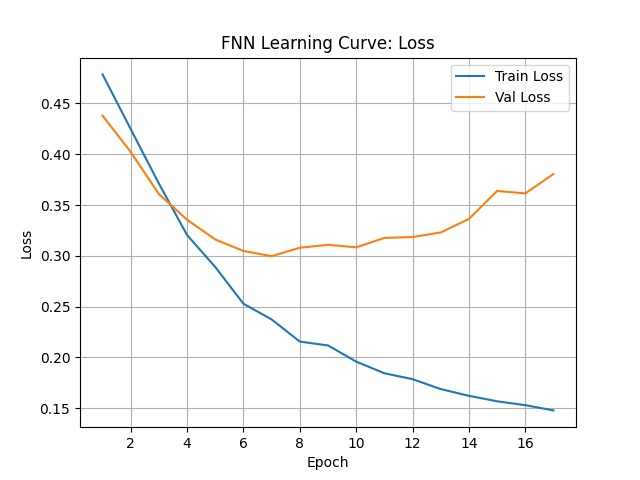
\includegraphics[width=\textwidth]{images/Supervised_Results/FNN_learning_curve_loss.jpg}
    \caption{Loss Learning Curve - FNN}
    \label{fig:fnn-loss}
\end{minipage}
\end{figure}

\subsection*{Additional Models Considered}

In addition to the CNN-RNN and FNN models a Random Forest classifier was also used. However, due to its underperformance and lack of generalizability, we omit detailed results for the Random Forest model.